% !TeX program = xelatex
% 配套题面资源 302-question-facsimiles.pdf 应与本文件置于同一目录。
\documentclass[UTF8,a4paper,zihao=-4,fontset=fandol,oneside]{ctexrep}
\usepackage[margin=21mm]{geometry}
\usepackage{graphicx,xcolor}
\usepackage[hidelinks,bookmarksopen=true]{hyperref}
\definecolor{muted}{HTML}{465766}
\setcounter{tocdepth}{1}
\setlength{\parindent}{0pt}
\raggedbottom
\newcommand{\questionclip}[1]{%
  \par\noindent\includegraphics[page=#1,width=\linewidth,height=.60\textheight,keepaspectratio]{302-question-facsimiles.pdf}\par}
\newcommand{\question}[5]{%
  \par\addvspace{.65\baselineskip}\noindent
  \begin{minipage}{\linewidth}
    \textbf{#1 年第 #2 题}\enspace #3\hfill{\small\textcolor{muted}{原卷 PDF 第 #4 页}}\par
    \smallskip #5
  \end{minipage}\par}

\title{302 数学二分节真题集}
\author{按《工科数学分析基础》第三版上册大纲编排}
\date{2009--2026 年全国硕士研究生招生考试}
\begin{document}
\maketitle
\chapter*{使用说明}
收录 18 份数学二原卷共 408 题。正文依教材上册四章 19 节编排，共 236 题；其余 172 题按知识领域列在附录。
每节内按选择、填空、解答分组，每组按年份与原题号排列。跨节题按主要考点归类，保留整道题。涉及弧长、旋转曲面面积等微元法应用的题目归入第三章第四节，曲率公式题另列附录。
每题注明年份、原题号、考点及题面所在的原卷 PDF 页码。题面取自逐年原卷，保留原有公式、选项与图形。源文件与配套题面 PDF 放在同一目录，LaTeX 从该资源逐题排版。
\tableofcontents

\chapter{函数、极限、连续}

\section{集合、映射与函数}

\noindent\textcolor{muted}{教材 PDF 第 24 页起，收录 1 题。}\par

\subsection*{选择题（1 题）}
\question{2024}{3}{函数的奇偶性}{1}{\questionclip{347}}

\section{数列的极限}

\noindent\textcolor{muted}{教材 PDF 第 41 页起，收录 10 题。}\par

\subsection*{选择题（5 题）}
\question{2012}{3}{数列与部分和的收敛}{1}{\questionclip{74}}
\question{2017}{3}{收敛数列的性质}{1}{\questionclip{189}}
\question{2022}{6}{递推数列的性质}{1}{\questionclip{306}}
\question{2023}{3}{递推数列与无穷小比较}{1}{\questionclip{325}}
\question{2024}{4}{数列极限的敛散性}{1}{\questionclip{348}}

\subsection*{填空题（1 题）}
\question{2012}{10}{和式型数列极限与夹逼准则}{2}{\questionclip{81}}

\subsection*{解答题（4 题）}
\question{2011}{19}{调和和式与数列收敛}{3}{\questionclip{67}}
\question{2012}{21}{实根构成的数列极限}{4}{\questionclip{92}}
\question{2013}{20}{不等式约束下的数列极限}{3}{\questionclip{114}}
\question{2018}{21}{递推数列的收敛与极限}{4}{\questionclip{230}}

\section{函数的极限}

\noindent\textcolor{muted}{教材 PDF 第 60 页起，收录 5 题。}\par

\subsection*{填空题（4 题）}
\question{2011}{9}{函数极限}{1}{\questionclip{57}}
\question{2013}{9}{指数型函数极限}{2}{\questionclip{103}}
\question{2019}{9}{指数型函数极限}{1}{\questionclip{241}}
\question{2022}{11}{指数型函数极限}{2}{\questionclip{311}}

\subsection*{解答题（1 题）}
\question{2011}{15}{两处函数极限与参数}{2}{\questionclip{63}}

\section{无穷小量与无穷大量}

\noindent\textcolor{muted}{教材 PDF 第 77 页起，收录 23 题。}\par

\subsection*{选择题（14 题）}
\question{2009}{2}{等价无穷小}{1}{\questionclip{2}}
\question{2011}{1}{三角函数的等价无穷小}{1}{\questionclip{49}}
\question{2012}{1}{渐近线条数}{1}{\questionclip{72}}
\question{2013}{1}{三角无穷小的比较}{1}{\questionclip{95}}
\question{2014}{1}{幂次与无穷小阶}{1}{\questionclip{118}}
\question{2014}{2}{渐近线的判定}{1}{\questionclip{119}}
\question{2016}{1}{无穷小量的阶}{1}{\questionclip{164}}
\question{2019}{1}{正切函数的同阶无穷小}{1}{\questionclip{233}}
\question{2020}{1}{积分形式的无穷小比阶}{1}{\questionclip{256}}
\question{2021}{1}{变上限积分的无穷小阶}{1}{\questionclip{279}}
\question{2022}{1}{等价无穷小的性质}{1}{\questionclip{301}}
\question{2023}{1}{斜渐近线}{1}{\questionclip{323}}
\question{2025}{4}{无穷小比阶}{1}{\questionclip{370}}
\question{2026}{1}{等价无穷小求系数}{1}{\questionclip{389}}

\subsection*{填空题（5 题）}
\question{2010}{10}{曲线的渐近线}{2}{\questionclip{35}}
\question{2016}{9}{斜渐近线}{2}{\questionclip{172}}
\question{2017}{9}{斜渐近线}{2}{\questionclip{195}}
\question{2023}{11}{等价无穷小求系数}{2}{\questionclip{333}}
\question{2025}{12}{斜渐近线}{2}{\questionclip{378}}

\subsection*{解答题（4 题）}
\question{2012}{15}{同阶无穷小与参数}{2}{\questionclip{86}}
\question{2013}{15}{三角乘积的等价无穷小}{2}{\questionclip{109}}
\question{2015}{15}{等价无穷小求参数}{2}{\questionclip{155}}
\question{2020}{15}{斜渐近线}{2}{\questionclip{270}}

\section{连续函数}

\noindent\textcolor{muted}{教材 PDF 第 86 页起，收录 8 题。}\par

\subsection*{选择题（8 题）}
\question{2009}{1}{可去间断点}{1}{\questionclip{1}}
\question{2010}{1}{无穷间断点}{1}{\questionclip{25}}
\question{2015}{2}{由极限定义的函数及间断点}{1}{\questionclip{142}}
\question{2015}{3}{分段函数连续性与参数}{1}{\questionclip{143}}
\question{2017}{1}{分段函数的连续条件}{1}{\questionclip{187}}
\question{2018}{3}{分段函数和的连续性}{1}{\questionclip{212}}
\question{2020}{2}{第二类间断点}{1}{\questionclip{257}}
\question{2024}{1}{间断点个数}{1}{\questionclip{345}}

\chapter{一元函数微分学及其应用}

\section{导数的概念}

\noindent\textcolor{muted}{教材 PDF 第 108 页起，收录 8 题。}\par

\subsection*{选择题（5 题）}
\question{2010}{3}{曲线相切}{1}{\questionclip{27}}
\question{2011}{2}{导数定义与极限}{1}{\questionclip{50}}
\question{2018}{2}{原点处的可导性}{1}{\questionclip{211}}
\question{2021}{2}{分段函数的可导性与极值}{1}{\questionclip{280}}
\question{2025}{7}{可导的等价条件}{2}{\questionclip{373}}

\subsection*{填空题（1 题）}
\question{2009}{9}{切线方程}{2}{\questionclip{10}}

\subsection*{解答题（2 题）}
\question{2022}{17}{由极限求导数}{2}{\questionclip{317}}
\question{2025}{18}{由极限判断可导性}{3}{\questionclip{384}}

\section{求导的基本法则}

\noindent\textcolor{muted}{教材 PDF 第 121 页起，收录 28 题。}\par

\subsection*{选择题（6 题）}
\question{2012}{2}{乘积求导}{1}{\questionclip{73}}
\question{2013}{2}{隐函数求导与极限}{1}{\questionclip{96}}
\question{2021}{3}{圆柱体的相关变化率}{1}{\questionclip{281}}
\question{2023}{5}{隐函数求导}{1}{\questionclip{327}}
\question{2024}{2}{参数方程求导与导数定义}{1}{\questionclip{346}}
\question{2026}{6}{反函数与变上限积分求导}{1}{\questionclip{394}}

\subsection*{填空题（20 题）}
\question{2009}{12}{隐函数求导}{2}{\questionclip{13}}
\question{2010}{11}{对数函数的高阶导数}{2}{\questionclip{36}}
\question{2010}{13}{相关变化率}{2}{\questionclip{38}}
\question{2012}{9}{隐函数求导}{2}{\questionclip{80}}
\question{2013}{10}{反函数求导}{2}{\questionclip{104}}
\question{2013}{12}{参数曲线的法线}{2}{\questionclip{106}}
\question{2014}{10}{奇偶性、周期性与求导}{2}{\questionclip{127}}
\question{2014}{12}{极坐标曲线的切线}{2}{\questionclip{129}}
\question{2015}{9}{隐函数求导}{2}{\questionclip{149}}
\question{2015}{10}{高阶导数}{2}{\questionclip{150}}
\question{2016}{13}{动点距离的相关变化率}{2}{\questionclip{176}}
\question{2017}{10}{参数方程求导}{2}{\questionclip{196}}
\question{2019}{10}{参数曲线切线的截距}{1}{\questionclip{242}}
\question{2019}{13}{高阶导数}{2}{\questionclip{245}}
\question{2020}{9}{参数方程的导数}{2}{\questionclip{264}}
\question{2021}{12}{参数方程求导}{2}{\questionclip{290}}
\question{2022}{12}{隐函数的二阶导数}{2}{\questionclip{312}}
\question{2023}{14}{隐函数曲线的法线}{2}{\questionclip{336}}
\question{2024}{14}{高阶导数}{2}{\questionclip{358}}
\question{2025}{14}{隐函数与参数方程求导}{2}{\questionclip{380}}

\subsection*{解答题（2 题）}
\question{2010}{17}{参数方程的二阶导数}{3}{\questionclip{42}}
\question{2018}{20}{面积的相关变化率}{3}{\questionclip{229}}

\section{微分}

\noindent\textcolor{muted}{教材 PDF 第 140 页起，收录 0 题。}\par
本节在所收原卷中没有以该节为主考点的题目。

\section{微分中值定理及其应用}

\noindent\textcolor{muted}{教材 PDF 第 147 页起，收录 12 题。}\par

\subsection*{选择题（2 题）}
\question{2014}{5}{L'Hospital 法则与函数极限}{1}{\questionclip{122}}
\question{2017}{2}{由可导条件推断中值点}{1}{\questionclip{188}}

\subsection*{填空题（1 题）}
\question{2018}{9}{反正切差的极限与中值定理}{2}{\questionclip{218}}

\subsection*{解答题（9 题）}
\question{2009}{21}{Lagrange 中值定理}{4}{\questionclip{22}}
\question{2010}{21}{两段区间上的中值定理}{4}{\questionclip{46}}
\question{2013}{18}{奇函数与中值定理}{3}{\questionclip{112}}
\question{2015}{21}{切线与中值定理证明}{4}{\questionclip{161}}
\question{2017}{15}{变上限积分的未定式极限}{2}{\questionclip{201}}
\question{2017}{19}{Rolle 定理与方程的根}{3}{\questionclip{205}}
\question{2019}{21}{中值定理与导数估计}{4}{\questionclip{253}}
\question{2023}{21}{极值条件与二阶中值结论}{4}{\questionclip{343}}
\question{2024}{21}{中值定理与导数估计}{3}{\questionclip{365}}

\section{Taylor定理及其应用}

\noindent\textcolor{muted}{教材 PDF 第 161 页起，收录 9 题。}\par

\subsection*{选择题（4 题）}
\question{2018}{1}{指数型极限与展开}{1}{\questionclip{210}}
\question{2020}{4}{由幂级展开求高阶导数值}{1}{\questionclip{259}}
\question{2021}{5}{二次 Taylor 多项式}{1}{\questionclip{283}}
\question{2022}{3}{二阶展开与极限}{1}{\questionclip{303}}

\subsection*{填空题（1 题）}
\question{2026}{12}{局部展开求函数极限}{2}{\questionclip{400}}

\subsection*{解答题（4 题）}
\question{2009}{15}{展开求极限}{3}{\questionclip{16}}
\question{2014}{15}{变上限积分与局部展开}{2}{\questionclip{132}}
\question{2016}{15}{三角函数展开求极限}{2}{\questionclip{178}}
\question{2021}{17}{局部展开求极限}{2}{\questionclip{295}}

\section{函数性态的研究}

\noindent\textcolor{muted}{教材 PDF 第 171 页起，收录 25 题。}\par

\subsection*{选择题（12 题）}
\question{2011}{3}{驻点个数}{1}{\questionclip{51}}
\question{2014}{3}{凹凸性与弦线}{1}{\questionclip{120}}
\question{2015}{4}{由二阶导数图像判定拐点}{1}{\questionclip{144}}
\question{2016}{4}{由导函数图像判断性态}{1}{\questionclip{167}}
\question{2018}{4}{凹凸性与积分平均值}{1}{\questionclip{213}}
\question{2019}{2}{拐点坐标}{1}{\questionclip{234}}
\question{2020}{6}{由导数不等式判断函数比值}{1}{\questionclip{261}}
\question{2021}{4}{单调性与零点个数}{1}{\questionclip{282}}
\question{2023}{6}{积分函数的最小值}{1}{\questionclip{328}}
\question{2023}{7}{极值点与拐点的参数条件}{2}{\questionclip{329}}
\question{2025}{2}{极值点和拐点的定义}{1}{\questionclip{368}}
\question{2026}{5}{单调性、极值与凹凸性}{1}{\questionclip{393}}

\subsection*{填空题（2 题）}
\question{2009}{13}{区间最值}{2}{\questionclip{14}}
\question{2018}{10}{拐点及其切线}{2}{\questionclip{219}}

\subsection*{解答题（11 题）}
\question{2010}{15}{变上限积分的单调性与极值}{2}{\questionclip{40}}
\question{2011}{16}{参数曲线的极值和拐点}{2}{\questionclip{64}}
\question{2012}{20}{用函数性态证明不等式}{3}{\questionclip{91}}
\question{2015}{19}{函数零点的个数}{3}{\questionclip{159}}
\question{2016}{16}{含绝对值的积分与最小值}{2}{\questionclip{179}}
\question{2017}{18}{隐函数的极值}{3}{\questionclip{204}}
\question{2018}{18}{构造函数证明不等式}{3}{\questionclip{227}}
\question{2019}{15}{求导与函数极值}{2}{\questionclip{247}}
\question{2021}{18}{凹凸区间与渐近线}{3}{\questionclip{296}}
\question{2022}{21}{二阶导数与凹凸性}{4}{\questionclip{321}}
\question{2025}{21}{导函数单调与函数凹凸性}{3}{\questionclip{387}}

\chapter{一元函数积分学及其应用}

\section{定积分的概念、存在条件与性质}

\noindent\textcolor{muted}{教材 PDF 第 189 页起，收录 11 题。}\par

\subsection*{选择题（4 题）}
\question{2012}{4}{定积分比较}{1}{\questionclip{75}}
\question{2018}{5}{定积分估计与比较}{1}{\questionclip{214}}
\question{2021}{7}{定积分与 Riemann 和}{1}{\questionclip{285}}
\question{2022}{7}{比较定积分大小}{2}{\questionclip{307}}

\subsection*{填空题（4 题）}
\question{2016}{10}{三角和式极限}{2}{\questionclip{173}}
\question{2024}{15}{速度的积分平均值}{2}{\questionclip{359}}
\question{2025}{13}{和式极限与定积分定义}{2}{\questionclip{379}}
\question{2026}{15}{函数的积分平均值}{2}{\questionclip{403}}

\subsection*{解答题（3 题）}
\question{2010}{16}{积分比较与数列极限}{2}{\questionclip{41}}
\question{2014}{19}{定积分保序与比较}{3}{\questionclip{136}}
\question{2020}{20}{积分中值定理}{3}{\questionclip{275}}

\section{微积分基本公式与基本定理}

\noindent\textcolor{muted}{教材 PDF 第 203 页起，收录 11 题。}\par

\subsection*{选择题（4 题）}
\question{2009}{6}{变上限积分的图像}{1、2}{\questionclip{6}\questionclip{7}}
\question{2013}{3}{变上限积分的连续性与可导性}{1}{\questionclip{97}}
\question{2016}{2}{分段函数的原函数}{1}{\questionclip{165}}
\question{2023}{2}{分段函数的原函数}{1}{\questionclip{324}}

\subsection*{填空题（3 题）}
\question{2015}{11}{变上限积分求导}{2}{\questionclip{151}}
\question{2016}{12}{变上限积分与高阶导数}{2}{\questionclip{175}}
\question{2023}{15}{积分关系求函数值}{2}{\questionclip{337}}

\subsection*{解答题（4 题）}
\question{2016}{21}{原函数、平均值与零点}{4}{\questionclip{184}}
\question{2018}{16}{变上限积分与平均值}{2}{\questionclip{225}}
\question{2020}{16}{变上限积分求导与连续性}{2}{\questionclip{271}}
\question{2026}{18}{变上限积分的导数与连续性}{2}{\questionclip{406}}

\section{两种基本积分法}

\noindent\textcolor{muted}{教材 PDF 第 214 页起，收录 14 题。}\par

\subsection*{选择题（3 题）}
\question{2011}{6}{定积分的对称换元}{1}{\questionclip{54}}
\question{2020}{3}{反三角函数的换元积分}{1}{\questionclip{258}}
\question{2022}{2}{定积分计算}{1}{\questionclip{302}}

\subsection*{填空题（6 题）}
\question{2009}{11}{含参数积分与分部积分}{2}{\questionclip{12}}
\question{2017}{11}{定积分计算}{2}{\questionclip{197}}
\question{2017}{13}{三角函数的定积分}{2}{\questionclip{199}}
\question{2018}{11}{有理函数的积分}{2}{\questionclip{220}}
\question{2020}{10}{换元计算定积分}{2}{\questionclip{265}}
\question{2022}{13}{有理函数的定积分}{2}{\questionclip{313}}

\subsection*{解答题（5 题）}
\question{2009}{16}{对数函数的不定积分}{3}{\questionclip{17}}
\question{2017}{17}{不定积分计算}{3}{\questionclip{203}}
\question{2018}{15}{换元与分部积分}{2}{\questionclip{224}}
\question{2019}{16}{不定积分计算}{2}{\questionclip{248}}
\question{2025}{17}{定积分计算}{3}{\questionclip{383}}

\section{定积分的应用}

\noindent\textcolor{muted}{教材 PDF 第 233 页起，收录 25 题。}\par

\subsection*{选择题（3 题）}
\question{2017}{6}{速度图像与追及距离}{1}{\questionclip{192}}
\question{2025}{6}{克服引力做功}{1}{\questionclip{372}}
\question{2026}{4}{连续分布质点的引力}{1}{\questionclip{392}}

\subsection*{填空题（8 题）}
\question{2010}{12}{极坐标曲线弧长}{2}{\questionclip{37}}
\question{2011}{11}{平面曲线弧长}{1}{\questionclip{59}}
\question{2013}{11}{极坐标曲线围成的面积}{2}{\questionclip{105}}
\question{2014}{13}{细棒的质心}{2}{\questionclip{130}}
\question{2019}{12}{对数曲线的弧长}{2}{\questionclip{244}}
\question{2020}{12}{水压力的微元法}{2}{\questionclip{267}}
\question{2022}{15}{极坐标曲线围成的面积}{2}{\questionclip{315}}
\question{2023}{12}{由积分表示的曲线弧长}{2}{\questionclip{334}}

\subsection*{解答题（14 题）}
\question{2010}{18}{液体质量的积分模型}{3}{\questionclip{43}}
\question{2011}{20}{旋转体容积与抽水做功}{3}{\questionclip{68}}
\question{2012}{17}{切线围成的面积与旋转体积}{2}{\questionclip{88}}
\question{2013}{16}{两个旋转体的体积关系}{2}{\questionclip{110}}
\question{2013}{21}{弧长与平面图形的形心}{4}{\questionclip{115}}
\question{2014}{20}{递推函数围成的面积}{3}{\questionclip{137}}
\question{2015}{16}{旋转体积的比值}{2}{\questionclip{156}}
\question{2016}{20}{旋转体积和表面积}{3}{\questionclip{183}}
\question{2019}{19}{分段面积与极限}{3}{\questionclip{251}}
\question{2020}{18}{函数关系与旋转体积}{3}{\questionclip{273}}
\question{2021}{19}{弧长与旋转曲面面积}{3}{\questionclip{297}}
\question{2023}{19}{无界区域的面积与旋转体积}{3}{\questionclip{341}}
\question{2024}{19}{旋转体积及其最大值}{3}{\questionclip{363}}
\question{2026}{20}{拐点与无界旋转体积}{2}{\questionclip{408}}

\section{反常积分}

\noindent\textcolor{muted}{教材 PDF 第 244 页起，收录 13 题。}\par

\subsection*{选择题（7 题）}
\question{2010}{4}{反常积分审敛}{1}{\questionclip{28}}
\question{2013}{4}{分段函数的反常积分}{1}{\questionclip{98}}
\question{2015}{1}{反常积分的收敛判别}{1}{\questionclip{141}}
\question{2016}{3}{反常积分敛散性}{1}{\questionclip{166}}
\question{2019}{3}{反常积分审敛}{1}{\questionclip{235}}
\question{2022}{5}{反常积分的收敛参数}{1}{\questionclip{305}}
\question{2024}{7}{非负函数的反常积分审敛}{1}{\questionclip{351}}

\subsection*{填空题（6 题）}
\question{2009}{10}{反常积分求参数}{2}{\questionclip{11}}
\question{2011}{12}{无穷区间上的积分}{2}{\questionclip{60}}
\question{2014}{9}{无穷区间上的反常积分}{2}{\questionclip{126}}
\question{2021}{11}{无穷区间上的积分}{2}{\questionclip{289}}
\question{2025}{11}{反常积分求参数}{2}{\questionclip{377}}
\question{2026}{11}{反常积分的收敛参数}{2}{\questionclip{399}}

\chapter{常微分方程}

\section{几类简单的微分方程}

\noindent\textcolor{muted}{教材 PDF 第 262 页起，收录 17 题。}\par

\subsection*{选择题（1 题）}
\question{2010}{2}{一阶线性方程解的关系}{1}{\questionclip{26}}

\subsection*{填空题（5 题）}
\question{2011}{10}{一阶线性方程初值问题}{1}{\questionclip{58}}
\question{2012}{12}{一阶微分方程初值问题}{2}{\questionclip{83}}
\question{2016}{11}{由特解确定一阶线性方程}{2}{\questionclip{174}}
\question{2024}{13}{一阶微分方程}{2}{\questionclip{357}}
\question{2025}{15}{一阶微分方程初值问题}{2}{\questionclip{381}}

\subsection*{解答题（11 题）}
\question{2009}{18}{降阶方程与旋转体积}{3}{\questionclip{19}}
\question{2011}{18}{由切线倾角建立微分方程}{3}{\questionclip{66}}
\question{2014}{16}{可分离变量方程与极值}{2}{\questionclip{133}}
\question{2015}{20}{Newton 冷却模型}{3}{\questionclip{160}}
\question{2017}{21}{由切线和法线条件建立方程}{4}{\questionclip{207}}
\question{2019}{17}{一阶线性方程与旋转体积}{2}{\questionclip{249}}
\question{2020}{21}{由面积比建立微分方程}{4}{\questionclip{276}}
\question{2021}{20}{一阶方程与距离最值}{3}{\questionclip{298}}
\question{2022}{18}{一阶方程与曲线弧长}{3}{\questionclip{318}}
\question{2023}{17}{由切线截距建立一阶方程}{3}{\questionclip{339}}
\question{2026}{21}{二阶微分方程降阶}{2}{\questionclip{409}}

\section{高阶线性微分方程}

\noindent\textcolor{muted}{教材 PDF 第 284 页起，收录 16 题。}\par

\subsection*{选择题（6 题）}
\question{2011}{4}{非齐次方程的特解形式}{1}{\questionclip{52}}
\question{2017}{4}{常系数非齐次方程特解}{1}{\questionclip{190}}
\question{2019}{4}{由通解确定方程系数}{1}{\questionclip{236}}
\question{2023}{4}{常系数方程解的有界性}{1}{\questionclip{326}}
\question{2025}{3}{常系数方程与反常积分收敛}{1}{\questionclip{369}}
\question{2026}{2}{非齐次方程的解的结构}{1}{\questionclip{390}}

\subsection*{填空题（6 题）}
\question{2010}{9}{三阶常系数齐次方程}{2}{\questionclip{34}}
\question{2013}{13}{非齐次方程的特解与初值}{2}{\questionclip{107}}
\question{2015}{12}{常系数齐次方程与极值条件}{2}{\questionclip{152}}
\question{2020}{13}{齐次方程初值问题与积分}{2}{\questionclip{268}}
\question{2021}{15}{常系数齐次方程的通解}{2}{\questionclip{293}}
\question{2022}{14}{三阶常系数齐次方程}{2}{\questionclip{314}}

\subsection*{解答题（4 题）}
\question{2009}{20}{分段求解微分方程}{4}{\questionclip{21}}
\question{2012}{19}{常系数方程与积分曲线拐点}{3}{\questionclip{90}}
\question{2016}{19}{二阶变系数线性方程}{3}{\questionclip{182}}
\question{2024}{18}{Euler 方程与定积分}{3}{\questionclip{362}}

\section{线性微分方程组（教材星号节）}

\noindent\textcolor{muted}{教材 PDF 第 310 页起，收录 0 题。}\par
本节在所收原卷中没有以该节为主考点的题目。

\appendix
\chapter{上册范围外真题}

\section{多元函数微分学}

\noindent\textcolor{muted}{收录 44 题。}\par

\subsection*{选择题（15 题）}
\question{2009}{3}{二元函数极值}{1}{\questionclip{3}}
\question{2010}{5}{隐函数偏导数}{1}{\questionclip{29}}
\question{2011}{5}{二元函数的极小值}{1}{\questionclip{53}}
\question{2012}{5}{偏导数符号与函数值比较}{1}{\questionclip{76}}
\question{2013}{5}{复合函数的偏导数}{1}{\questionclip{99}}
\question{2014}{6}{多元函数的最值位置}{1}{\questionclip{123}}
\question{2015}{5}{复合函数的偏导数}{1}{\questionclip{145}}
\question{2016}{6}{二元函数在原点的性质}{1}{\questionclip{169}}
\question{2017}{5}{偏导数与函数值比较}{1}{\questionclip{191}}
\question{2020}{5}{多元极限和偏导数}{1}{\questionclip{260}}
\question{2021}{6}{由复合函数条件求全微分}{1}{\questionclip{284}}
\question{2022}{4}{含变上限积分的偏导数}{1}{\questionclip{304}}
\question{2024}{5}{偏导数与可微性}{1}{\questionclip{349}}
\question{2025}{1}{隐函数偏导数}{1}{\questionclip{367}}
\question{2026}{3}{隐函数偏导数}{1}{\questionclip{391}}

\subsection*{填空题（11 题）}
\question{2012}{11}{复合函数求偏导}{2}{\questionclip{82}}
\question{2014}{11}{隐函数的全微分}{2}{\questionclip{128}}
\question{2015}{13}{隐函数的全微分}{2}{\questionclip{153}}
\question{2017}{12}{由全微分恢复二元函数}{2}{\questionclip{198}}
\question{2018}{13}{隐函数的偏导数}{2}{\questionclip{222}}
\question{2019}{11}{复合函数偏导数}{2}{\questionclip{243}}
\question{2020}{11}{二元函数的全微分}{2}{\questionclip{266}}
\question{2021}{13}{隐函数偏导数}{2}{\questionclip{291}}
\question{2023}{13}{隐函数偏导数}{2}{\questionclip{335}}
\question{2024}{12}{二元函数极值}{2}{\questionclip{356}}
\question{2026}{14}{全微分与复合求导}{2}{\questionclip{402}}

\subsection*{解答题（18 题）}
\question{2009}{17}{二阶偏导数}{3}{\questionclip{18}}
\question{2010}{19}{二阶偏导数与变量变换}{3}{\questionclip{44}}
\question{2011}{17}{复合函数的偏导数}{2}{\questionclip{65}}
\question{2012}{16}{二元函数极值}{2}{\questionclip{87}}
\question{2013}{19}{二元条件最值}{3}{\questionclip{113}}
\question{2014}{18}{复合函数偏导与方程变换}{3}{\questionclip{135}}
\question{2014}{21}{由偏导数恢复边界与旋转体积}{4}{\questionclip{138}}
\question{2015}{17}{二元函数极值}{2}{\questionclip{157}}
\question{2016}{17}{隐函数的无条件极值}{2}{\questionclip{180}}
\question{2017}{16}{复合函数的二阶偏导}{2}{\questionclip{202}}
\question{2018}{19}{多元约束最值}{3}{\questionclip{228}}
\question{2019}{20}{偏导数与方程变换}{3}{\questionclip{252}}
\question{2020}{17}{二元函数极值}{3}{\questionclip{272}}
\question{2022}{20}{由偏导数恢复二元函数及其极值}{3}{\questionclip{320}}
\question{2023}{18}{二元函数极值}{3}{\questionclip{340}}
\question{2024}{20}{偏导数与原函数}{3}{\questionclip{364}}
\question{2025}{19}{利用全微分求函数及极值}{3}{\questionclip{385}}
\question{2026}{19}{二元函数极值}{2}{\questionclip{407}}

\section{二重积分}

\noindent\textcolor{muted}{收录 30 题。}\par

\subsection*{选择题（10 题）}
\question{2009}{4}{交换积分次序}{1}{\questionclip{4}}
\question{2010}{6}{二重积分换序}{1}{\questionclip{30}}
\question{2012}{6}{二重积分与积分区域}{1}{\questionclip{77}}
\question{2013}{6}{象限区域上的二重积分符号}{1}{\questionclip{100}}
\question{2015}{6}{极坐标下的积分限}{1}{\questionclip{146}}
\question{2018}{6}{二重积分的次序变换}{1}{\questionclip{215}}
\question{2019}{5}{二重积分与积分区域}{1}{\questionclip{237}}
\question{2024}{6}{二重积分换序}{1}{\questionclip{350}}
\question{2025}{5}{二重积分交换次序}{1}{\questionclip{371}}
\question{2026}{7}{二重积分定义与对称性}{1}{\questionclip{395}}

\subsection*{填空题（2 题）}
\question{2011}{13}{极坐标二重积分}{2}{\questionclip{61}}
\question{2021}{14}{二重积分确定函数值}{2}{\questionclip{292}}

\subsection*{解答题（18 题）}
\question{2009}{19}{区域对称与二重积分}{3}{\questionclip{20}}
\question{2010}{20}{二重积分计算}{3}{\questionclip{45}}
\question{2011}{21}{含偏导数的二重积分}{4}{\questionclip{69}}
\question{2012}{18}{心形线区域上的二重积分}{3}{\questionclip{89}}
\question{2013}{17}{三角形区域上的二重积分}{2}{\questionclip{111}}
\question{2014}{17}{环形区域上的二重积分}{2}{\questionclip{134}}
\question{2015}{18}{二重积分计算}{3}{\questionclip{158}}
\question{2016}{18}{二重积分计算}{3}{\questionclip{181}}
\question{2017}{20}{二重积分计算}{3}{\questionclip{206}}
\question{2018}{17}{参数曲线围成区域上的积分}{3}{\questionclip{226}}
\question{2019}{18}{极坐标二重积分}{3}{\questionclip{250}}
\question{2020}{19}{二重积分计算}{3}{\questionclip{274}}
\question{2021}{21}{极坐标二重积分}{4}{\questionclip{299}}
\question{2022}{19}{二重积分计算}{3}{\questionclip{319}}
\question{2023}{20}{二重积分的变量代换}{4}{\questionclip{342}}
\question{2024}{17}{二重积分计算}{2}{\questionclip{361}}
\question{2025}{20}{二重积分计算}{3}{\questionclip{386}}
\question{2026}{17}{二重积分计算}{2}{\questionclip{405}}

\section{曲率与曲率圆}

\noindent\textcolor{muted}{收录 8 题。}\par

\subsection*{选择题（4 题）}
\question{2009}{5}{曲率圆与曲线性态}{1}{\questionclip{5}}
\question{2014}{4}{参数曲线的曲率半径}{1}{\questionclip{121}}
\question{2016}{5}{曲率、公切线与曲线位置}{1}{\questionclip{168}}
\question{2019}{6}{相切、曲率与二阶展开}{1}{\questionclip{238}}

\subsection*{填空题（4 题）}
\question{2012}{13}{曲率与点的坐标}{2}{\questionclip{84}}
\question{2018}{12}{参数曲线的曲率}{2}{\questionclip{221}}
\question{2024}{11}{曲率圆方程}{2}{\questionclip{355}}
\question{2026}{13}{隐式曲线的曲率半径}{2}{\questionclip{401}}

\section{线性代数}

\noindent\textcolor{muted}{收录 90 题。}\par

\subsection*{选择题（42 题）}
\question{2009}{7}{分块矩阵与伴随矩阵}{2}{\questionclip{8}}
\question{2009}{8}{矩阵相似与二次型}{2}{\questionclip{9}}
\question{2010}{7}{向量组的线性表示}{1}{\questionclip{31}}
\question{2010}{8}{实对称矩阵的相似}{1、2}{\questionclip{32}\questionclip{33}}
\question{2011}{7}{初等矩阵与逆矩阵}{1}{\questionclip{55}}
\question{2011}{8}{伴随矩阵与基础解系}{1}{\questionclip{56}}
\question{2012}{7}{向量组线性相关}{1}{\questionclip{78}}
\question{2012}{8}{相似矩阵与特征值}{1}{\questionclip{79}}
\question{2013}{7}{矩阵幂与相似}{1}{\questionclip{101}}
\question{2013}{8}{矩阵相似的充要条件}{1}{\questionclip{102}}
\question{2014}{7}{行列式计算}{1}{\questionclip{124}}
\question{2014}{8}{线性无关的充分必要条件}{1}{\questionclip{125}}
\question{2015}{7}{线性方程组有无穷多解}{1}{\questionclip{147}}
\question{2015}{8}{二次型的正交变换}{1}{\questionclip{148}}
\question{2016}{7}{相似矩阵的性质}{1}{\questionclip{170}}
\question{2016}{8}{二次型惯性指数}{1}{\questionclip{171}}
\question{2017}{7}{矩阵相似与对角化}{2}{\questionclip{193}}
\question{2017}{8}{矩阵运算}{2}{\questionclip{194}}
\question{2018}{7}{相似矩阵的判定}{1}{\questionclip{216}}
\question{2018}{8}{分块矩阵的秩}{2}{\questionclip{217}}
\question{2019}{7}{伴随矩阵与基础解系}{1}{\questionclip{239}}
\question{2019}{8}{特征值与二次型规范形}{1}{\questionclip{240}}
\question{2020}{7}{代数余子式与齐次方程组}{1}{\questionclip{262}}
\question{2020}{8}{特征向量与对角化}{2}{\questionclip{263}}
\question{2021}{8}{二次型的惯性指数}{1}{\questionclip{286}}
\question{2021}{9}{向量组的线性表示}{2}{\questionclip{287}}
\question{2021}{10}{初等变换与对角矩阵}{2}{\questionclip{288}}
\question{2022}{8}{矩阵的特征值}{2}{\questionclip{308}}
\question{2022}{9}{线性方程组解的讨论}{2}{\questionclip{309}}
\question{2022}{10}{向量组等价}{2}{\questionclip{310}}
\question{2023}{8}{伴随矩阵运算}{2}{\questionclip{330}}
\question{2023}{9}{二次型的规范形}{2}{\questionclip{331}}
\question{2023}{10}{向量的共同线性表示}{2}{\questionclip{332}}
\question{2024}{8}{矩阵运算}{2}{\questionclip{352}}
\question{2024}{9}{伴随矩阵和矩阵秩}{2}{\questionclip{353}}
\question{2024}{10}{矩阵的相似对角化}{2}{\questionclip{354}}
\question{2025}{8}{矩阵特征值的符号}{2}{\questionclip{374}}
\question{2025}{9}{矩阵初等行变换}{2}{\questionclip{375}}
\question{2025}{10}{矩阵秩与方程组的解}{2}{\questionclip{376}}
\question{2026}{8}{置换矩阵的性质}{1}{\questionclip{396}}
\question{2026}{9}{矩阵方程的可解性}{2}{\questionclip{397}}
\question{2026}{10}{矩阵恒等式与秩}{2}{\questionclip{398}}

\subsection*{填空题（18 题）}
\question{2009}{14}{相似矩阵与秩}{2}{\questionclip{15}}
\question{2010}{14}{行列式的性质}{2}{\questionclip{39}}
\question{2011}{14}{二次型的正惯性指数}{2}{\questionclip{62}}
\question{2012}{14}{伴随矩阵的行列式}{2}{\questionclip{85}}
\question{2013}{14}{代数余子式与行列式}{2}{\questionclip{108}}
\question{2014}{14}{二次型的负惯性指数}{2}{\questionclip{131}}
\question{2015}{14}{矩阵多项式与特征值}{2}{\questionclip{154}}
\question{2016}{14}{等价矩阵与矩阵秩}{2}{\questionclip{177}}
\question{2017}{14}{特征向量与参数}{2}{\questionclip{200}}
\question{2018}{14}{矩阵的特征值}{2}{\questionclip{223}}
\question{2019}{14}{代数余子式}{2}{\questionclip{246}}
\question{2020}{14}{行列式计算}{2}{\questionclip{269}}
\question{2021}{16}{行列式多项式的系数}{2}{\questionclip{294}}
\question{2022}{16}{初等变换与逆矩阵的迹}{2}{\questionclip{316}}
\question{2023}{16}{线性方程组的可解条件}{2}{\questionclip{338}}
\question{2024}{16}{向量组线性相关}{2}{\questionclip{360}}
\question{2025}{16}{线性方程组通解}{2}{\questionclip{382}}
\question{2026}{16}{矩阵乘积与二次型}{2}{\questionclip{404}}

\subsection*{解答题（30 题）}
\question{2009}{22}{特征向量与线性无关}{4}{\questionclip{23}}
\question{2009}{23}{二次型的规范形}{4}{\questionclip{24}}
\question{2010}{22}{非齐次线性方程组}{4}{\questionclip{47}}
\question{2010}{23}{实对称矩阵的正交对角化}{4}{\questionclip{48}}
\question{2011}{22}{向量组的线性表示}{4}{\questionclip{70}}
\question{2011}{23}{实对称矩阵的特征值}{4}{\questionclip{71}}
\question{2012}{22}{行列式与线性方程组}{4}{\questionclip{93}}
\question{2012}{23}{二次型的秩与正交变换}{4}{\questionclip{94}}
\question{2013}{22}{矩阵方程}{4}{\questionclip{116}}
\question{2013}{23}{二次型矩阵与标准形}{4}{\questionclip{117}}
\question{2014}{22}{基础解系与矩阵方程}{4}{\questionclip{139}}
\question{2014}{23}{矩阵相似的证明}{4}{\questionclip{140}}
\question{2015}{22}{矩阵方程与矩阵幂}{4}{\questionclip{162}}
\question{2015}{23}{相似矩阵与对角化}{4}{\questionclip{163}}
\question{2016}{22}{线性方程组与通解}{4}{\questionclip{185}}
\question{2016}{23}{矩阵方程与列向量表示}{4}{\questionclip{186}}
\question{2017}{22}{矩阵秩与方程组通解}{4}{\questionclip{208}}
\question{2017}{23}{二次型正交化}{4}{\questionclip{209}}
\question{2018}{22}{二次型规范形}{4}{\questionclip{231}}
\question{2018}{23}{矩阵的初等列变换}{4}{\questionclip{232}}
\question{2019}{22}{等价向量组}{4}{\questionclip{254}}
\question{2019}{23}{矩阵相似与相似变换}{4}{\questionclip{255}}
\question{2020}{22}{二次型的合同变换}{4}{\questionclip{277}}
\question{2020}{23}{相似对角化的判断}{4}{\questionclip{278}}
\question{2021}{22}{矩阵的相似对角化}{4}{\questionclip{300}}
\question{2022}{22}{二次型的正交变换}{4}{\questionclip{322}}
\question{2023}{22}{线性变换的相似对角化}{4}{\questionclip{344}}
\question{2024}{22}{方程组同解与正交对角化}{3}{\questionclip{366}}
\question{2025}{22}{矩阵合同与正交对角化}{3}{\questionclip{388}}
\question{2026}{22}{极大线性无关组与矩阵幂}{3}{\questionclip{410}}

\end{document}
